% ============================================================================
%  seminar.tex  --  Beamer deck + study reference
%  Paper : Jamali, Sadabadi, Davari, "A Cyber-Resilient Secondary Frequency
%          Control Framework for VSG-Controlled Microgrids With GFM IBRs",
%          IEEE Trans. Ind. Electron., vol. 73, no. 3, pp. 3992-4006, Mar. 2026
%  Build : pdflatex seminar.tex   (run twice)
%  Needs : Fig1_Controller_Comparison.png, Fig2_Money_Slide.png,
%          Fig3_Power_Sharing.png, Fig4_Tradeoff_Curve.png in the same folder
%          (a grey placeholder box is printed if a PNG is missing)
% ============================================================================
\documentclass[aspectratio=169,9pt]{beamer}

\usepackage[T1]{fontenc}
\usepackage[utf8]{inputenc}
\IfFileExists{lmodern.sty}{\usepackage{lmodern}}{}
\usepackage{amsmath,amssymb,bm}
\usepackage{booktabs,array}
\usepackage{graphicx}
\usepackage{tikz}
\usetikzlibrary{arrows.meta,calc}

% ---------------------------------------------------------------- theme
\usetheme{default}
\usecolortheme{dove}
\setbeamercolor{structure}{fg=black}
\setbeamercolor{frametitle}{fg=black}
\setbeamerfont{frametitle}{series=\bfseries,size=\large}
\setbeamercolor{block title}{fg=black,bg=black!8}
\setbeamercolor{block body}{fg=black,bg=black!3}
\setbeamercolor{block title alerted}{fg=black,bg=black!14}
\setbeamercolor{block body alerted}{fg=black,bg=black!3}
\setbeamercolor{block title example}{fg=black,bg=black!8}
\setbeamercolor{block body example}{fg=black,bg=black!3}
\setbeamertemplate{navigation symbols}{}
\setbeamertemplate{itemize items}[circle]
\setbeamertemplate{footline}{\hfill\insertframenumber\hspace{0.5em}\vspace{0.4em}}
\setbeamerfont{block title}{size=\small,series=\bfseries}
\setbeamersize{text margin left=0.7cm,text margin right=0.7cm}
\setlength{\leftmargini}{1.1em}
\renewcommand{\arraystretch}{1.18}

% ---------------------------------------------------------------- macros
\newcommand{\bbK}{\mathbb{K}}
\newcommand{\bbH}{\mathbb{H}}
\newcommand{\dd}{\mathrm{d}}
\newcommand{\Emat}{E}
\newcommand{\abs}[1]{\left|#1\right|}
\newcommand{\norm}[1]{\left\|#1\right\|}
\newcommand{\Linf}{\mathcal{L}_\infty}
\newcommand{\Lone}{\mathcal{L}_1}
\newcommand{\ones}{\mathbf{1}}
\newcommand{\figorbox}[2]{\IfFileExists{#1}{\includegraphics[width=#2\linewidth]{#1}}{\fbox{\parbox{\dimexpr#2\linewidth-2\fboxsep-2\fboxrule\relax}{\centering\footnotesize\vspace{1.2cm}Missing figure: \detokenize{#1}\vspace{1.2cm}}}}}

\title[Cyber-resilient secondary control]{Cyber-Resilient Secondary Frequency Control\\for VSG-Controlled Microgrids}
\subtitle{Paper review, derivations, and an independent reduced-order check}
\author[Aayush]{Aayush}
\institute[NIT Goa]{National Institute of Technology Goa}
\date{\today}

\begin{document}

% =========================================================================
\begin{frame}[plain]
\titlepage
\vspace{-0.3cm}
{\footnotesize M.~Jamali, M.~S.~Sadabadi, M.~Davari, \emph{IEEE Trans. Industrial Electronics}, vol.~73, no.~3, pp.~3992--4006, Mar.~2026.}
\end{frame}

% =========================================================================
\begin{frame}[t]{Roadmap}
\begin{columns}[T]
\column{0.5\textwidth}
\textbf{Part I -- Context}
\begin{itemize}\footnotesize
\item Motivation, gap, contributions
\item Model: swing equations on a graph
\item Attack model and assumptions
\end{itemize}
\textbf{Part II -- Controller and theory}
\begin{itemize}\footnotesize
\item The ancillary-state (``leaky'') controller
\item Lur'e representation (derived)
\item Lemma 1 (Lyapunov), Lemma 2 (small gain)
\item Theorem 1 and the convex program
\end{itemize}
\textbf{Part III -- The paper's evidence}
\begin{itemize}\footnotesize
\item Test microgrid, Table I, Cases 1--5, PHIL
\end{itemize}
\column{0.5\textwidth}
\textbf{Part IV -- My independent check (Octave)}
\begin{itemize}\footnotesize
\item What was simulated, and what was \emph{not}
\item Closed-form steady state (derived)
\item Results, Figs.~1--4, trade-off in $H$
\item What the numbers do and do not support
\end{itemize}
\textbf{Part V -- Critique}
\begin{itemize}\footnotesize
\item Strengths, limitations, open questions
\end{itemize}
\textbf{Appendix (reference)}
\begin{itemize}\footnotesize
\item Notation, Q\&A, how to run the code, formula sheet
\end{itemize}
\vspace{0.3cm}
\begin{alertblock}{Honesty note}\footnotesize
Slides marked \textbf{[mine]} are my own analysis or simulation, not claims of the paper.
\end{alertblock}
\end{columns}
\end{frame}

% =========================================================================
%  PART I
% =========================================================================
\begin{frame}[t]{Motivation: low inertia $+$ a networked control layer}
\begin{columns}[T]
\column{0.56\textwidth}
\footnotesize
\begin{itemize}
\item \textbf{Real threat.} 2015 Ukraine grid attack [2]; a regional-supply attack on the UK is estimated at \pounds11.6--85.5\,bn of losses across sectors [3].
\item \textbf{IBR-only islanded microgrids} have almost no physical inertia, so frequency moves fast after any disturbance, a cyberattack included [4,8].
\item Grid-forming (GFM) IBRs set voltage and frequency; there is no physical link between frequency and power, so \emph{droop} or \emph{VSG} (emulated swing equation) creates one.
\item \textbf{Secondary control} restores frequency and shares power, but it runs over a communication network: a natural attack surface (false data injection, FDI) [6,19].
\item Prior work: mostly \emph{detection} [16--18] (no mitigation), or resilient designs that are droop-based and ignore transient stability [20--22].
\end{itemize}
\column{0.42\textwidth}
\begin{block}{Paper's goal}\footnotesize
Keep GFM-IBR frequencies inside a safe set under bounded FDI on the secondary-control channel,
\begin{itemize}
\item \emph{without} detecting or isolating the attack,
\item \emph{with} a quantitative bound on the tolerable attack size.
\end{itemize}
\end{block}
\begin{block}{Why IBR-only?}\footnotesize
Worst case: lowest inertia, so the largest attack impact and the most stealthy-attack exposure [4]. Adding SGs only helps.
\end{block}
\end{columns}
\end{frame}

% =========================================================================
\begin{frame}[t]{Contributions claimed by the paper}
\footnotesize
\begin{enumerate}
\item \textbf{Resilient controller with ancillary states.} Unlike DAI-type secondary control [13,24], it tolerates \emph{bounded} FDI on the control inputs and does not need to identify the attack.
\item \textbf{Transient \emph{and} steady-state resilience} for VSG-controlled microgrids, unlike [22,25]. Tolerates, rather than detects, the attack.
\item \textbf{System-theoretic certificate.} Lur'e representation $+$ constrained input--output stability, with a performance index built on the elementwise $\Linf$ vector norm and the $\Lone$ system (gain-matrix) norm. A convex program returns the \emph{maximum attack bound} $\bar\delta$ that keeps $\norm{\omega}_{\Linf}\le\bar y$ (IEEE Std 2030.8-2018).
\end{enumerate}
\vspace{0.2cm}
\begin{columns}[T]
\column{0.5\textwidth}
\begin{exampleblock}{Validation in the paper}\footnotesize
\begin{itemize}
\item MATLAB: 4 GFM IBRs, full-order (LCL, inner PI loops, DC link, delays).
\item Compared with DAI [24], robust [14], primal-dual [47].
\item PHIL tests at LAPES (RTDS NovaCor, SEMIKRON, dSPACE).
\end{itemize}
\end{exampleblock}
\column{0.5\textwidth}
\begin{block}{Where the novelty sits}\footnotesize
Not in a new plant model. It is (i) the leak/ancillary-state structure, a ``retrofit'' of integral control, and (ii) the \emph{analysis machinery} that turns resilience into a computable number.
\end{block}
\end{columns}
\end{frame}

% =========================================================================
\begin{frame}[t]{Model: swing equations on a graph (Sec.~II-A)}
\footnotesize
Graph $\mathcal G(\mathcal V,\mathcal E)$: $n$ IBRs, $l$ lines, incidence matrix $E\in\mathbb R^{n\times l}$.
\begin{columns}[T]
\column{0.52\textwidth}
\textbf{Per unit} $i$ (eq.~2):
\[\dot\theta_i=\omega_i,\qquad m_i\dot\omega_i=-d_i\omega_i+P^{\rm net}_i-P_i+u_i\]
\textbf{Lossless power flow, const.\ voltage} (eq.~3):
\[P_i=\sum_{(i,j)\in\mathcal E} b_{ij}V_iV_j\sin(\theta_i-\theta_j)\]
\textbf{Stacked form} (eq.~4):
\[\dot\theta=\omega,\qquad M\dot\omega=-D\omega+P^{\rm net}-E\Phi\sin(E^{\!T}\theta)+u\]
with $M{=}\mathrm{diag}(m_i)$, $D{=}\mathrm{diag}(d_i)$, $\Phi{=}\mathrm{diag}(\Phi_k)$, $\Phi_k=b_{ij}V_iV_j$ for line $k=(i,j)$.
\column{0.46\textwidth}
\begin{block}{Why $E\Phi\sin(E^T\theta)$?}
$(E^T\theta)_k=\theta_i-\theta_j$ is the angle across line $k$; the flow $\Phi_k\sin(\cdot)$ leaves node $i$ and enters node $j$. Summing over lines gives $P=E\Phi\sin(E^T\theta)$, and $\ones^TE=0$, so \emph{network flows sum to zero}.
\end{block}
\begin{alertblock}{Assumption 1 (security)}
There is an equilibrium $\theta^*$ with $\psi^*:=E^T\theta^*\in(-\pi/2,\pi/2)^l$. It is never unique: shifting all angles by a common constant gives another one.
\end{alertblock}
\end{columns}
\vspace{0.1cm}
{\scriptsize Modelling choices stated by the paper: lossless lines, constant voltage magnitudes, swing model valid for \emph{system-level} frequency control; inner voltage/current loops are abstracted away.}
\end{frame}

% =========================================================================
\begin{frame}[t]{Attack model and assumptions (Sec.~II-B,C)}
\footnotesize
\begin{columns}[T]
\column{0.55\textwidth}
\textbf{Actuation attack} (eq.~5), additive on the secondary command:
\[M\dot\omega=-D\omega+P^{\rm net}-E\Phi\sin(E^T\theta)+u+\delta_u\]
\textbf{Computational attack} on the controller state: $\delta_\xi$ (added in eq.~7c).
\begin{alertblock}{Assumption 2}
$\norm{\delta_u}_{\Linf}\le\bar\delta_u$: ``unknown but bounded'', and \emph{independent of the state trajectory}. The same is assumed for $\delta_\xi$.
\end{alertblock}
\textbf{Why bounded?} Unbounded or wildly out-of-range injections would be flagged by anomaly detectors, and actuators saturate. Stealthy attacks stay inside operating margins [32--34].
\column{0.43\textwidth}
\begin{block}{Control objective}
Synchronism $|\omega_i-\omega_k|=0$ under the constraint $\norm{\omega}_{\Linf}\le\bar y$, where $\bar y$ is the maximum deviation allowed by IEEE Std 2030.8-2018.
\end{block}
\begin{exampleblock}{Out of scope (acknowledged)}
Attacks on measurements or neighbour exchanges; unbounded attacks; state-dependent attacks. DoS and replay are only \emph{simulated} (Case 3), not proved.
\end{exampleblock}
\end{columns}
\end{frame}

% =========================================================================
%  PART II
% =========================================================================
\begin{frame}[t]{The proposed controller: an ancillary state with a leak (Sec.~III-A)}
\footnotesize
\begin{columns}[T]
\column{0.5\textwidth}
\textbf{Control law} (eq.~6):
\[u=\beta\bbK\xi,\qquad \dot\xi=-\bbH\xi-\beta\bbK^{T}\omega\]
$\xi\in\mathbb R^n$ ancillary state, $\bbK$ interconnection matrix, $\bbH\succ0$ (the \textbf{leak}), $\beta>0$ scalar gain.
\vspace{0.1cm}

\textbf{Transfer function} (derive from 6b): $\xi(s)=-(sI+\bbH)^{-1}\beta\bbK^T\omega(s)$, so
\[u(s)=-\beta^2\,\bbK(sI+\bbH)^{-1}\bbK^T\,\omega(s)\]
Scalar case: $u=-\dfrac{\beta^2K^2}{s+H}\,\omega$, a \textbf{low-pass} (lag) filter.
\begin{itemize}
\item $H=0$: pure integrator, classical secondary control (DAI-type).
\item $H>0$: no integral action, so $\omega=0$ is no longer enforced.
\end{itemize}
\column{0.48\textwidth}
\begin{block}{Topology is set by $\bbK,\bbH$}
Dense $\bbK,\bbH$: centralised. $\bbK$ = Laplacian of a communication graph and $\bbH$ diagonal: \emph{distributed} (each IBR talks to its neighbours only).
\end{block}
\begin{block}{``Retrofitting''}
Adds states to the standard integral loop; can be carried over to other frequency models of GFM IBRs.
\end{block}
\begin{alertblock}{[mine] DC gain of the controller}
Setting $s=0$: $u=-\dfrac{\beta^2K^2}{H}\omega$. With the paper's numbers ($\beta{=}100$, $K{=}2$, $H{=}150$): $\boxed{-266.7\,\omega}$, to be compared with the physical damping $d_i=13\,880$.
\end{alertblock}
\end{columns}
\end{frame}

% =========================================================================
\begin{frame}[t]{Closed loop with attacks, and its equilibrium (eq.~7)}
\footnotesize
\begin{align*}
\dot\theta&=\omega &&(7a)\\
M\dot\omega&=-D\omega+P^{\rm net}-E\Phi\sin(E^T\theta)+\beta\bbK\xi+\delta_u &&(7b)\\
\dot\xi&=-\bbH\xi-\beta\bbK^T\omega+\delta_\xi &&(7c)
\end{align*}
\begin{columns}[T]
\column{0.5\textwidth}
\textbf{Attack-free equilibrium.} Setting $\dot{(\cdot)}=0$ gives $\omega=0$, then $\bbH\xi=0\Rightarrow\xi=0$, then $P^{\rm net}=E\Phi\sin(E^T\theta^*)$. So $x^*=[\theta^{*T},0,0]^T$.
\column{0.48\textwidth}
\begin{alertblock}{[mine] A subtle point}
$x^*$ has $\xi^*=0$ \emph{only if} $P^{\rm net}\in\mathrm{Im}(E\Phi\sin(\cdot))$, i.e.\ no net power mismatch. After a load change the leaky controller needs $\xi\neq0$ to push back, and then $\omega^*\neq0$. The theory is for the attack-induced deviation from $x^*$, not a load step.
\end{alertblock}
\end{columns}
\end{frame}

% =========================================================================
\begin{frame}[t]{Lur'e representation: derivation of (8)--(9)}
\footnotesize
\begin{columns}[T]
\column{0.58\textwidth}
Let $\tilde\theta=\theta-\theta^*$, $q=E^T\tilde\theta$, $\psi^*=E^T\theta^*$. Expand the sine about $\psi^*$:
\[\sin(\psi^*+q)=\sin\psi^*+\mathrm{diag}(\cos\psi^*)\,q+\nu(q)\]
\[\nu(q)=\sin(\psi^*+q)-\sin\psi^*-\mathrm{diag}(\cos\psi^*)q\qquad(9d)\]
Use $P^{\rm net}=E\Phi\sin\psi^*$ in (7b) to cancel the constant part:
\[M\dot\omega=-D\omega-E\Phi\,\mathrm{diag}(\cos\psi^*)E^T\tilde\theta+\beta\bbK\xi-E\Phi\,\nu(q)+\delta_u\]
With $x=[\tilde\theta;\omega;\xi]$: $\dot x=Ax+B_\nu\nu(q)+B_\delta\delta$, $y=\omega=C_yx$, $q=C_qx$, $\delta=[\delta_u;\delta_\xi]$,
\[A=\begin{bmatrix}0&I&0\\-M^{-1}E\Phi\,\mathrm{diag}(\cos\psi^*)E^T&-M^{-1}D&\beta M^{-1}\bbK\\0&-\beta\bbK^T&-\bbH\end{bmatrix}\]
$B_\nu=[0;-M^{-1}E\Phi;0]$, $B_\delta=\begin{bmatrix}0&0\\M^{-1}&0\\0&I\end{bmatrix}$, $C_y=[0\ I\ 0]$, $C_q=[E^T\ 0\ 0]$.
\column{0.4\textwidth}
\begin{center}
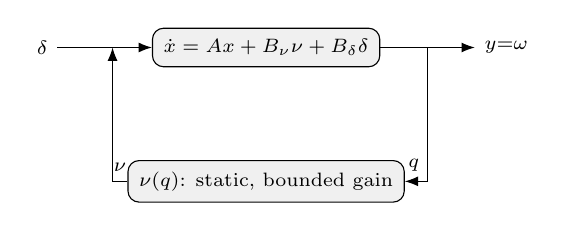
\begin{tikzpicture}[>=Latex,box/.style={draw,rounded corners,fill=black!6,inner sep=4pt,font=\scriptsize}]
\node[box] (lti) at (0,0) {$\dot x=Ax+B_\nu\nu+B_\delta\delta$};
\node[box] (nl) at (0,-1.7) {$\nu(q)$: static, bounded gain};
\draw[->] ($(lti.west)+(-1.2,0)$) node[left]{\scriptsize$\delta$} -- (lti.west);
\draw[->] (lti.east) -- ++(1.2,0) node[right]{\scriptsize$y{=}\omega$};
\draw[->] ($(lti.east)+(0.6,0)$) |- node[pos=0.8,above]{\scriptsize$q$} (nl.east);
\draw[->] (nl.west) -| node[pos=0.25,above]{\scriptsize$\nu$} ($(lti.west)+(-0.5,0)$);
\end{tikzpicture}
\end{center}
\begin{block}{Why do it?}
The \emph{linear} block carries all the dynamics and the attack; the \emph{only} nonlinearity is a bounded static feedback, so classical input--output (small-gain) tools apply.
\end{block}
\end{columns}
\end{frame}

% =========================================================================
\begin{frame}[t]{The nonlinear element: bounding $\nu_i(q_i)$ (Sec.~III-C)}
\footnotesize
\begin{columns}[T]
\column{0.52\textwidth}
\textbf{Paper:} $\nu_i(q_i)=\sin(\psi_i^*+q_i)-\sin\psi_i^*-\cos(\psi_i^*)q_i$, with gain
\[\gamma_{\nu_i}=\sup_{q_i}\left|\frac{\nu_i(q_i)}{q_i}\right|,\quad\gamma_\nu=\mathrm{diag}(\gamma_{\nu_i}),\quad \norm{\nu}_{\Linf}\le\gamma_\nu\norm{q}_{\Linf}\ (13)\]
\textbf{[mine] A closed-form bound.} Taylor with Lagrange remainder: for some $\zeta$ between $0$ and $q_i$,
\[\nu_i(q_i)=-\tfrac12\sin(\psi_i^*+\zeta)\,q_i^2\ \Longrightarrow\ \left|\frac{\nu_i}{q_i}\right|\le\frac{|q_i|}{2}\]
so, restricted to $|q_i|\le\bar q_i$: $\ \gamma_{\nu_i}(\bar q_i)\le\bar q_i/2$.
\column{0.46\textwidth}
\begin{block}{Reading it}
\begin{itemize}
\item The nonlinear gain is \emph{small for small angle deviations} and grows with $\bar q$; this is why Fig.~12(a) plots $\gamma_\nu$ against $\bar q$.
\item Over the whole line, $|\nu_i/q_i|\le 2$ trivially, but that is far too conservative.
\item The condition $|\psi^*_i|+\bar q_i\le\pi$ keeps the angle inside one sine period.
\end{itemize}
\end{block}
\begin{alertblock}{Subtle}
$\gamma_\nu$ is valid only while $|q|\le\bar q$ is already known. That is circular unless a continuation (bootstrap) argument is added; see Theorem~1.
\end{alertblock}
\end{columns}
\end{frame}

% =========================================================================
\begin{frame}[t]{Lemma 1: the linear block is stable (Lyapunov + LaSalle)}
\footnotesize
\begin{columns}[T]
\column{0.55\textwidth}
Let $L_\psi:=E\Phi\,\mathrm{diag}(\cos\psi^*)E^T$ (symmetric, weighted Laplacian since $\cos\psi^*>0$). Candidate:
\[V(x)=\tfrac12\tilde\theta^TL_\psi\tilde\theta+\tfrac12\omega^TM\omega+\tfrac12\xi^T\xi\qquad(14)\]
\textbf{Derivative along $\dot x=Ax$} (the pieces):
\begin{align*}
\dot V&=\tilde\theta^TL_\psi\omega+\omega^T\!\bigl(-L_\psi\tilde\theta-D\omega+\beta\bbK\xi\bigr)+\xi^T\!\bigl(-\beta\bbK^T\omega-\bbH\xi\bigr)\\
&=-\omega^TD\omega-\xi^T\bbH\xi+\underbrace{\beta\omega^T\bbK\xi-\beta\xi^T\bbK^T\omega}_{=0}
\end{align*}
\[\boxed{\dot V=-\omega^TD\omega-\xi^T\bbH\xi\le0}\qquad(15)\]
The coupling terms cancel because the same $\beta\bbK$ appears in $u$ and in $\dot\xi$: a skew-symmetric (power-conserving) interconnection. LaSalle: $\dot V\equiv0\Rightarrow\omega=0,\xi=0\Rightarrow L_\psi\tilde\theta=0$.
\column{0.43\textwidth}
\begin{alertblock}{[mine] Two precision remarks}
\begin{enumerate}
\item $L_\psi$ is \emph{singular} ($L_\psi\ones=0$), so $V$ is only positive \emph{semi}definite in $\tilde\theta$; the claim ``$V>0\ \forall x\ne0$'' needs $\tilde\theta\perp\ones$. LaSalle gives $L_\psi\tilde\theta=0\Rightarrow\tilde\theta\in\mathrm{span}(\ones)$: stability is of $(q,\omega,\xi)=0$, i.e.\ \emph{synchronisation}, not of $\tilde\theta=0$.
\item The role of $\bbH\succ0$: it makes $\xi$ appear in $\dot V$. With $\bbH=0$, $\dot V$ only controls $\omega$; $\xi$ is free and nothing bounds it against $\delta_\xi$.
\end{enumerate}
\end{alertblock}
\end{columns}
\end{frame}

% =========================================================================
\begin{frame}[t]{Gain matrices and the $\Lone$ bound (eq.~1, 16, 17)}
\footnotesize
\begin{columns}[T]
\column{0.53\textwidth}
\textbf{Definition.} For a stable $G(s)$ with impulse responses $g_{ij}$: $\gamma_{G,ij}=\norm{G_{ij}}_{\Lone}=\int|g_{ij}(\tau)|\,\dd\tau$.
\vspace{0.1cm}

\textbf{Why it bounds the peak.} For $y_i=\sum_j g_{ij}*\delta_j$ (zero initial state):
\[|y_i(t)|\le\sum_j\int_0^t|g_{ij}(\tau)|\,|\delta_j(t-\tau)|\,\dd\tau\le\sum_j\gamma_{G,ij}\norm{\delta_j}_{\Linf}\]
\[\Rightarrow\ \norm{y}_{\Linf}\le\gamma_G\,\norm{\delta}_{\Linf}\ \text{(elementwise)}\]
The bound is \emph{tight} for the worst-case bounded input (peak-to-peak gain).

\textbf{Applied to Lur'e blocks} with $y=G_{y,\delta}\delta+G_{y,\nu}\nu$ and $q=E^T\!\int\!y$-type relation, $\gamma_{q,\cdot}=E^{T}_{|\cdot|}\,\gamma_{y,\cdot}$ (16):
\begin{align*}
\norm{y}_{\Linf}&\le\gamma_{y,\delta}\norm{\delta}_{\Linf}+\gamma_{y,\nu}\norm{\nu}_{\Linf}&(17a)\\
\norm{q}_{\Linf}&\le E^T_{|\cdot|}\bigl(\gamma_{y,\delta}\norm{\delta}_{\Linf}+\gamma_{y,\nu}\norm{\nu}_{\Linf}\bigr)&(17b)
\end{align*}
\column{0.45\textwidth}
\begin{block}{Why $\Linf$ / $\Lone$?}
Grid-code limits are \emph{peak} limits on frequency. $\Linf$ captures the worst-case peak regardless of the energy of the disturbance; its induced system norm is exactly the $\Lone$ norm of the impulse response, which is what makes the bound computable.
\end{block}
\begin{block}{$E^T_{|\cdot|}$}
The matrix of absolute values of the entries of $E^T$. Needed because the bounds are \emph{elementwise} and signs cannot cancel in a worst case.
\end{block}
\end{columns}
\end{frame}

% =========================================================================
\begin{frame}[t]{Lemma 2: BIBO stability by a small-gain (Neumann) argument}
\footnotesize
\begin{columns}[T]
\column{0.58\textwidth}
Put $\Gamma:=E^T_{|\cdot|}\gamma_{y,\nu}\gamma_\nu\in\mathbb R^{l\times l}_{\ge0}$. Insert (13) into (17b):
\begin{align*}
\norm{q}_{\Linf}&\le E^T_{|\cdot|}\gamma_{y,\delta}\norm{\delta}_{\Linf}+\Gamma\norm{q}_{\Linf}\\
\Rightarrow\ (I-\Gamma)\norm{q}_{\Linf}&\le E^T_{|\cdot|}\gamma_{y,\delta}\norm{\delta}_{\Linf}\qquad(18)
\end{align*}
If the Perron--Frobenius eigenvalue satisfies $\lambda_{\max}(\Gamma)<1$, the Neumann series converges:
\[(I-\Gamma)^{-1}=\sum_{k\ge0}\Gamma^k\ \ge0\ \ (\text{elementwise})\]
Multiplying (18) by a nonnegative matrix preserves the inequality:
\begin{align*}
\norm{q}_{\Linf}&\le(I-\Gamma)^{-1}E^T_{|\cdot|}\gamma_{y,\delta}\norm{\delta}_{\Linf}\\
\norm{\nu}_{\Linf}&\le\gamma_\nu\norm{q}_{\Linf}
\end{align*}
\[\boxed{\norm{y}_{\Linf}\le\gamma\,\norm{\delta}_{\Linf}},\quad\gamma=\gamma_{y,\delta}+\gamma_{y,\nu}\gamma_\nu(I-\Gamma)^{-1}E^T_{|\cdot|}\gamma_{y,\delta}\ \ (20)\]
\column{0.4\textwidth}
\begin{block}{Interpretation}
$\gamma$ is a finite, nonnegative \emph{closed-loop gain matrix} from the attack $\delta$ to the frequency: a bounded input gives a bounded output (BIBO). The factor $(I-\Gamma)^{-1}$ is the amplification from the angle-feedback loop; it blows up as $\lambda_{\max}(\Gamma)\to1$.
\end{block}
\begin{alertblock}{Typos in print (cosmetic)}
Eqs.~(16)--(19) mix $\gamma_{q,\nu}$, $\gamma_{y,V\nu}$ and $E^T_{|\cdot|}\gamma_{y,\nu}$ for the same object. The structure above is the consistent reading.
\end{alertblock}
\end{columns}
\end{frame}

% =========================================================================
\begin{frame}[t]{Theorem 1 and the resilience optimisation (Sec.~IV)}
\footnotesize
\begin{columns}[T]
\column{0.57\textwidth}
\begin{block}{Theorem 1 (paper)}
If there exist $\bar\delta,\bar q\ge0$ with
\[E^T_{|\cdot|}\bigl(\gamma_{y,\delta}\bar\delta+\gamma_{y,\nu}\gamma_\nu\bar q\bigr)\le\bar q,\qquad\gamma_{y,\delta}\bar\delta+\gamma_{y,\nu}\gamma_\nu\bar q\le\bar y\ (22)\]
then every attack with $\norm{\delta}_{\Linf}\le\bar\delta$ gives $\norm{\omega}_{\Linf}\le\bar y$.
\end{block}
\textbf{Optimisation (23):} $\ \max_{\bar q\ge0,\ \bar\delta\ge0}\ \bar\delta\ \ \text{s.t. (22)}$, the largest tolerable attack. Inputs: topology $E$, gain matrices, $\bar y$. Needs $|\psi_i^*|+\bar q_i\le\pi$.

\textbf{Role of $\beta$ (Figs.~3, 12).} Raising $\beta$ raises the tolerable $\bar\delta$ (but too large a $\beta$ degrades transients, more oscillation).
\column{0.41\textwidth}
\begin{alertblock}{[mine] Gaps worth knowing}
\begin{enumerate}
\item \textbf{Bootstrap.} (22) assumes $|q|\le\bar q$ to define $\gamma_\nu(\bar q)$. A continuation argument ($q(0)=0$, continuity, ``first time $|q|=\bar q$'') is needed to close it; the paper says only ``from Lemma 2 and (17)''.
\item \textbf{Convexity.} With $\gamma_\nu$ fixed, (23) is a linear program. Since $\gamma_\nu$ depends on $\bar q$, convexity is asserted via [41] rather than shown.
\item \textbf{Conservatism} is admitted by the authors as future work.
\end{enumerate}
\end{alertblock}
\end{columns}
\end{frame}

% =========================================================================
%  PART III
% =========================================================================
\begin{frame}[t]{The paper's evidence: test system and parameters (Sec.~V, Table I)}
\footnotesize
\begin{columns}[T]
\column{0.5\textwidth}
\textbf{Test microgrid.} 4 GFM IBRs as VSGs, 3 lines (Fig.~4, 13); full-order model: inner PI voltage/current loops, LCL filters, DC-link dynamics, delay blocks; $\omega_0=2\pi60$.
\vspace{0.1cm}

\textbf{Controller:} $\beta=100$, $\bbK=2I_4$, $\bbH=150\,I_4$.
\vspace{0.1cm}

\begin{tabular}{@{}ll@{}}
\toprule
\textbf{Parameter} & \textbf{Value}\\
\midrule
$d_i/m_i$ & $13\,880/1000$\\
$K_{PV}/K_{IV}$ & $0.01/1.8$\\
$K_{PC}/K_{IC}$ & $1/33$\\
LCL & $R_f{=}0.05\,\Omega$, $L_f{=}1.5$\,mH, $C_f{=}50\,\mu$F\\
 & $R_c{=}0.1\,\Omega$, $L_c{=}1.35$\,mH; $R_g{=}0.03\,\Omega$, $L_g{=}0.35$\,mH\\
Lines & $R_{1..3}{=}0.25,0.4,0.35\,\Omega$; $L_{1..3}{=}0.3,1.8,1.8$\,mH\\
\bottomrule
\end{tabular}
\column{0.48\textwidth}
\begin{alertblock}{[mine] What the paper does \emph{not} give}
The line susceptances $\Phi$, the equilibrium angles $\psi^*$, the numerical limit $\bar y$, and the value of the computed $\bar\delta$ are not tabulated. Any reproduction of the reduced model must \emph{assume} them.
\end{alertblock}
\begin{block}{PHIL rig (LAPES, Georgia Southern)}
RTDS NovaCor real-time simulator, Spitzenberger\,\&\,Spies power amplifiers (Aurora link), SEMIKRON converter with AC/DC filters, dSPACE MicroLabBox. Each GFM IBR is tested as the ``hardware of interest'' against the rest of the microgrid as the ``model of interest''.
\end{block}
\end{columns}
\end{frame}

% =========================================================================
\begin{frame}[t]{The paper's evidence: case studies}
\footnotesize
\begin{center}
\scriptsize
\begin{tabular}{@{}p{0.06\linewidth}p{0.40\linewidth}p{0.50\linewidth}@{}}
\toprule
\textbf{Case} & \textbf{Scenario} & \textbf{Reported outcome}\\
\midrule
1 & $\delta_u=[8\sin t,\ 7\sin(t{+}\tfrac\pi2),$ $5\sin(t{+}\tfrac\pi3),\ 3\sin(t{+}\tfrac\pi2)]$ and $\delta_\xi=1.25\,\delta_u$ (computational), $t=5$--$12$\,s & Frequencies stay synchronised; steady frequency slightly ($<0.2\%$) below 1\,p.u., attributed to the VSG \emph{governor}. DAI [24], robust [14], primal-dual [47] lose synchrony and power sharing. \\
2 & Case 1 with a 10\% decrease in LCL, line, $\Phi$, $M$, $D$ & Still synchronised, power shared proportionally. \\
3 & Replay attack: delayed replay of recorded signals (20 samples), from $5$\,s & Stable, zero steady-state frequency error; \emph{no stability proof} for replay. \\
4 & $\delta=[10\sin10t,\ 12\sin(15t{+}\tfrac\pi2),$ $5\sin(5t{+}\tfrac\pi3),\ 6\sin(12t{+}\tfrac\pi2)]$ (faster, larger) & Still resilient; faster attacks hurt more. \\
5 & Mixed grid: an SG at IBR\,\#2 and a GFL IBR at IBR\,\#4, load\,\#4 doubled for $6$--$9$\,s & Stable, acceptable performance. \\
\midrule
PHIL & Cases 1--3 and Case 5 replicated on hardware & Close agreement with simulation. \\
\bottomrule
\end{tabular}
\end{center}
{\scriptsize Fig.~12: nonlinear gain vs.\ $\bar q$ and maximum attack size for $\beta=100$; Fig.~3: maximum bound $\bar\Delta$ vs.\ $\beta$.}
\end{frame}

% =========================================================================
%  PART IV
% =========================================================================
\begin{frame}[t]{[mine] Independent check: what was simulated, and what was not}
\footnotesize
\begin{columns}[T]
\column{0.55\textwidth}
\textbf{States} $x=[\theta(4);\,\omega(4);\,\xi(4)]$: the closed loop (7) exactly, on the path graph 1--2--3--4 (3 lines).
\begin{itemize}
\item $M=1000\,I$, $D=13\,880\,I$ (Table I); $\beta=100$, $K=2$, $H=150$.
\item \textbf{Assumed} (not in the paper): $\Phi=2\times10^4\,I_3$, $\psi^*=[0.10,-0.05,0.08]^T$, $P^{\rm net}=E\Phi\sin\psi^*$ (makes $\theta^*$ an exact equilibrium).
\item Attacks from Case 1, window $5$--$12$\,s; \textbf{sinusoidal} (paper) and \textbf{constant-bias} (for analysis): $\delta_u=[8,7,5,3]$, $\delta_\xi=[10,8.75,6.25,3.75]$.
\item Load step: $-2000$\,W at node 4 at $t=2$\,s, no attack.
\end{itemize}
\textbf{Three controllers:} primary only ($\beta=0$), proposed ($H=150$), pure integrator ($H=0$, $\beta=100$).
\column{0.43\textwidth}
\begin{block}{Why the swing level?}
The theory (Lur'e form, Lemmas 1--2, Theorem 1) is derived \emph{only} from (7). Simulating (7) tests the control law and the theory in isolation, without inner-loop tuning, PWM and filter dynamics.
\end{block}
\begin{alertblock}{What this check cannot say}
Anything about LCL filters, inner loops, DC-link dynamics, delays, resistive lines, or hardware. The paper's \emph{dramatic} baseline failures are in the full-order model; I did not reproduce those, nor the baselines [14], [24], [47] themselves ($H=0$ is a stand-in for a pure integrator, not for DAI).
\end{alertblock}
\end{columns}
\end{frame}

% =========================================================================
\begin{frame}[t]{[mine] Derivation: steady state under constant bias attacks (leaky controller)}
\footnotesize
\begin{columns}[T]
\column{0.57\textwidth}
Take scalar gains $M,D,K,H$ (as in the paper's test), constant $\delta_u,\delta_\xi$ and a constant net power mismatch $\Delta P$ at a node. Assume a \emph{synchronous} steady state $\omega_i\equiv\omega_s$, $\dot\xi=0$.
\medskip

\textbf{(a) Sum the swing equations over nodes.} $\ones^TE=0$ removes all network flows:
\[0=-nD\omega_s+\beta K\textstyle\sum_i\xi_i+\sum_i\delta_{u,i}+\sum_i\Delta P_i\]
\textbf{(b) Each $\xi$ equation:} $0=-H\xi_i-\beta K\omega_s+\delta_{\xi,i}\Rightarrow\xi_i=\dfrac{\delta_{\xi,i}-\beta K\omega_s}{H}$.
\textbf{(c) Insert (b) into (a):}
\[\boxed{\ \omega_s=\frac{H\,(\bar\delta_u+\overline{\Delta P})+\beta K\,\bar\delta_\xi}{HD+\beta^2K^2}\ }\qquad(\text{bars}=\text{mean over nodes})\]
\column{0.41\textwidth}
\begin{block}{Limits}
\begin{itemize}
\item $\beta=0$: $\omega_s=(\bar\delta_u+\overline{\Delta P})/D$. No $\xi$, so $\delta_\xi$ has no effect.
\item $H\to\infty$: $\omega_s\to(\bar\delta_u+\overline{\Delta P})/D$ (controller switched off).
\item $\beta\to\infty$: $\omega_s\to\bar\delta_\xi/(\beta K)\to0$: why more $\beta$ helps (Fig.~3).
\end{itemize}
\end{block}
\begin{alertblock}{Valid only for $H>0$}
For $H=0$ each $\xi_i$ is a \emph{local} integrator, $\dot\xi_i=\delta_{\xi,i}-\beta K\omega_i$, which pins $\omega_i\to\delta_{\xi,i}/(\beta K)$ node by node. A synchronous steady state generally does not exist (next slides).
\end{alertblock}
\end{columns}
\end{frame}

% =========================================================================
\begin{frame}[t]{[mine] Numbers: closed form vs.\ simulation (constant bias, $t\in[11.5,12]$ s)}
\footnotesize
\begin{center}
\begin{tabular}{@{}lccc@{}}
\toprule
$\max_i|\omega_i|$ (rad/s) & Primary only & Proposed ($H{=}150$) & Pure integrator ($H{=}0$)\\
\midrule
$\delta_u$ only & $4.1\times10^{-4}$ & $4.1\times10^{-4}$ & $\approx0$ (rejected)\\
$\delta_\xi$ only & $0$ (no $\xi$) & $6.8\times10^{-4}$ & $4.7\times10^{-2}$\\
both & $4.1\times10^{-4}$ & $1.09\times10^{-3}$ & $4.7\times10^{-2}$\\
\midrule
Load $-2000$\,W, final $\omega$ & $-3.60\times10^{-2}$ & $-3.53\times10^{-2}$ & $\approx0$ (restored)\\
Sinusoidal attack (Case 1), peak & $5.6\times10^{-4}$ & $1.46\times10^{-3}$ & $4.0\times10^{-2}$\\
\bottomrule
\end{tabular}
\end{center}
\vspace{-0.1cm}
\begin{columns}[T]
\column{0.5\textwidth}
\textbf{Closed form (c) for $H=150$:} denominator $HD+\beta^2K^2=2.122\times10^6$.\\
$\delta_u$ only: $150\cdot5.75/2.122\!\times\!10^6=4.06\!\times\!10^{-4}$\\
$\delta_\xi$ only: $200\cdot7.1875/2.122\!\times\!10^6=6.77\!\times\!10^{-4}$\\
both: $2300/2.122\!\times\!10^6=1.084\!\times\!10^{-3}$\\
load: $150\cdot(-500)/2.122\!\times\!10^6=-3.53\!\times\!10^{-2}$
\column{0.48\textwidth}
{\scriptsize These match a separate Python/SciPy re-implementation of the same ODE; check them against your own Octave console output (the first block of \texttt{jamali\_vsg\_demo.m} prints exactly the constant-bias rows). The sinusoidal-peak row is a numerical value, not a closed form.}
\begin{exampleblock}{Reading the $H{=}0$ column}
$4.7\times10^{-2}$ is node 1 (individual nodes sit at $4.7,\,4.2,\,3.2,\,2.3\times10^{-2}$, not equal): synchrony is lost, as the paper describes for its baselines. Compare the uncoupled pin $\delta_{\xi,i}/(\beta K)=5.0,\,4.4,\,3.1,\,1.9\times10^{-2}$.
\end{exampleblock}
\end{columns}
\end{frame}

% =========================================================================
\begin{frame}[t]{[mine] What the leak does: dynamics and effective droop}
\footnotesize
\begin{columns}[T]
\column{0.5\textwidth}
\textbf{Common-mode characteristic polynomial} (scalar gains, network flow terms cancel in the mean):
\[M s^2+(D+MH)s+(DH+\beta^2K^2)=0\]
\begin{center}
\begin{tabular}{@{}lll@{}}
\toprule
 & polynomial / $M$ & poles ($s^{-1}$)\\
\midrule
$H{=}0$ & $s^2+13.88s+40$ & $-4.1,\,-9.8$\\
$H{=}150$ & $s^2+163.9s+2122$ & $-14.2,\,-149.7$\\
primary & $s+13.88$ & $-13.88$\\
\bottomrule
\end{tabular}
\end{center}
\textbf{Attack gain at $1$\,rad/s} ($\delta_\xi\to\omega$, common mode):\\
$|G|=\dfrac{\beta K}{|\,(Ms{+}D)(s{+}H)+\beta^2K^2|}$ gives $4.8\times10^{-3}$ ($H{=}0$) vs.\ $9.4\times10^{-5}$ ($H{=}150$): about $51\times$ attenuation per unit of common-mode $\delta_\xi$.
\column{0.48\textwidth}
\begin{block}{The leak = a small extra droop}
Below the corner $H=150$\,rad/s, far above the electromechanical band ($\sim$4--14\,s$^{-1}$), the controller behaves as a \emph{static} gain $u=-(\beta^2K^2/H)\omega$:
\[D_{\rm eff}=D+\frac{\beta^2K^2}{H}=13\,880+266.7\ (+1.9\%)\]
\end{block}
\begin{alertblock}{Consequence}
At $H=150$ the controller delivers resilience (about $50\times$ vs.\ $H{=}0$ on $\delta_\xi$) and gives back only 1.9\% of the load-step frequency error relative to primary control ($3.53$ vs.\ $3.60\times10^{-2}$\,rad/s). Almost all of the ``restoration'' has been traded away. The paper's own claim that the leak causes no problem rests on the governor explanation for the 0.2\% offset in the \emph{full} model, which I cannot test at swing level.
\end{alertblock}
\end{columns}
\end{frame}

% =========================================================================
\begin{frame}[t]{[mine] Fig.~1: three controllers under the paper's sinusoidal attack}
\begin{columns}[T]
\column{0.64\textwidth}
\figorbox{Fig1_Controller_Comparison.png}{1.0}
\column{0.34\textwidth}
\footnotesize
{\scriptsize Shaded: attack window $5$--$12$\,s.}
\begin{itemize}
\item Numerical peaks of $|\omega|$ during the attack: primary $5.6\times10^{-4}$, proposed $1.46\times10^{-3}$, $H{=}0$ $4.0\times10^{-2}$\,rad/s, i.e.\ the leaky controller is about $27\times$ better than the pure integrator and about $2.6\times$ \emph{worse} than having no secondary loop at all.
\item $H=0$: individual frequencies split during the attack; after $t=12$\,s they return to $0$, but $\xi$ and the angles settle at \emph{new} offsets (the integrator never forgets).
\item $H>0$: sync is kept, small ripple at the attack frequency.
\end{itemize}
\end{columns}
\end{frame}

% =========================================================================
\begin{frame}[t]{[mine] Fig.~2: proposed controller, normal $\to$ attack $\to$ normal}
\begin{columns}[T]
\column{0.62\textwidth}
\figorbox{Fig2_Money_Slide.png}{1.0}
\column{0.36\textwidth}
\footnotesize
\begin{itemize}
\item $0$--$5$\,s: at the equilibrium ($\omega=0$). $5$--$12$\,s: bounded response, peak $\sim10^{-3}$\,rad/s, i.e.\ $\sim4\times10^{-6}$ of $\omega_0=377$\,rad/s.
\item After $12$\,s: returns to $0$ within about a second (poles at $-14$ and $-150$\,s$^{-1}$), then stays: the leak forgets the attack.
\item Theory check: Lemma 1 ($\dot V\le0$) plus bounded inputs gives a bounded response, as seen.
\end{itemize}
\begin{alertblock}{Careful}\scriptsize
Peak $|\omega|\ll\bar y$ here does not by itself validate Theorem~1's \emph{bound}; that needs $\gamma$ matrices, which I did not compute.
\end{alertblock}
\end{columns}
\end{frame}

% =========================================================================
\begin{frame}[t]{[mine] Fig.~3: network power injections during the attack}
\begin{columns}[T]
\column{0.62\textwidth}
\figorbox{Fig3_Power_Sharing.png}{1.0}
\column{0.36\textwidth}
\footnotesize
\begin{itemize}
\item Plotted: $P_e=E\Phi\sin(E^T\theta)$, the net \emph{network injection} at each IBR.
\item This is \textbf{not} a proportional-power-sharing metric: that needs the droop/VSG ratios, and the paper shows it only in its full-order Figs.~5--11.
\item Use it to show that line flows stay far from the $\pm\Phi$ limit ($2\times10^4$\,W) during the attack, i.e.\ Assumption~1 is not threatened.
\end{itemize}
\begin{alertblock}{Do not claim}\scriptsize
``Power sharing remains proportional'' from this plot.
\end{alertblock}
\end{columns}
\end{frame}

% =========================================================================
\begin{frame}[t]{[mine] Why the pure integrator is the real hazard: differential-mode drift}
\footnotesize
\begin{columns}[T]
\column{0.54\textwidth}
With $H=0$ and diagonal $K$: $\dot\xi_i=\delta_{\xi,i}-\beta K\omega_i$. A synchronous steady state would need $\omega_i=\omega_s$ for all $i$, hence $\dot\xi_i=\delta_{\xi,i}-\beta K\omega_s$, which is nonzero for every node whose bias differs from the mean:
\begin{align*}
\delta_{\xi,i}-\bar\delta_\xi&=(+2.81,\,+1.56,\,-0.94,\,-3.44)\\
\dot u_i=\beta K\dot\xi_i&=(+563,\,+313,\,-188,\,-688)\ \text{W/s}
\end{align*}
So the $u_i$ would ramp linearly (wind-up). The system compromises: $\omega_i$ separate (values above), the angles slip at a constant rate instead:
\begin{center}
\begin{tabular}{@{}lccc@{}}
\toprule
 & $q_1$ & $q_2$ & $q_3$ (rad)\\
\midrule
$t=12$\,s (end of real attack) & 0.14 & 0.02 & 0.14\\
$t=80$\,s (attack continued) & 0.52 & 0.69 & 0.75\\
$t=200$\,s & 0.96 & 2.41 & 2.09\\
\bottomrule
\end{tabular}
\end{center}
{\scriptsize Numerical, $H=0$ and bias attack held on. For $H=150$ the angles stay at their equilibrium values $(0.10,-0.05,0.08)$.}
\column{0.44\textwidth}
\begin{block}{Reading it}
\begin{itemize}
\item In the 7\,s of the paper's scenario the damage is a frequency split of about $2.4\times10^{-2}$\,rad/s, small in absolute terms.
\item The structural issue is that the angle differences have \emph{no restoring equilibrium}: held long enough they pass $\pm\pi/2$ (Assumption~1) and synchronism is lost.
\item With the leak, $\xi_i=(\delta_{\xi,i}-\beta K\omega_s)/H$ is bounded, so $u_i$ is bounded, so the angles stay put.
\end{itemize}
\end{block}
\begin{exampleblock}{Optional extra experiment}
In \texttt{rhs\_func.m} change \texttt{t <= 12} to \texttt{t <= 300}; in \texttt{run\_sim.m} change the 12 in \texttt{breaks}; use the \texttt{'bias'} attack and \texttt{Tend = 300}. Compare $H=0$ vs.\ $150$.
\end{exampleblock}
\end{columns}
\end{frame}

% =========================================================================
\begin{frame}[t]{[mine] The resilience vs.\ restoration trade-off in $H$ (closed form)}
\footnotesize
\begin{columns}[T]
\column{0.5\textwidth}
From the boxed formula (both attacks, load step $-500$\,W per node on average):
\begin{align*}
\text{attack: }&A(H)=\frac{5.75\,H+1437.5}{13.88\,H+40}\ \text{mrad/s}\\
\text{load: }&L(H)=\frac{500\,H}{13.88\,H+40}\ \text{mrad/s}
\end{align*}
\begin{itemize}
\item $A$ falls monotonically from $35.9$ at $H\to0^+$ to $0.4143$ as $H\to\infty$; $L$ rises from $0$ to $36.0$.
\item They cross at $H^\dagger=\beta K\bar\delta_\xi/(|\overline{\Delta P}|-\bar\delta_u)\approx2.9$, not near the paper's $H=150$.
\item At $H=150$: $L=35.3$ ($98\%$ of the primary-only error), $A=1.08$.
\end{itemize}
\vspace{0.1cm}
{\scriptsize Numerical sweep (sinusoidal attack, node-1 peak) crosses between $H=3$ and $10$ as well.}
\column{0.48\textwidth}
\begin{center}
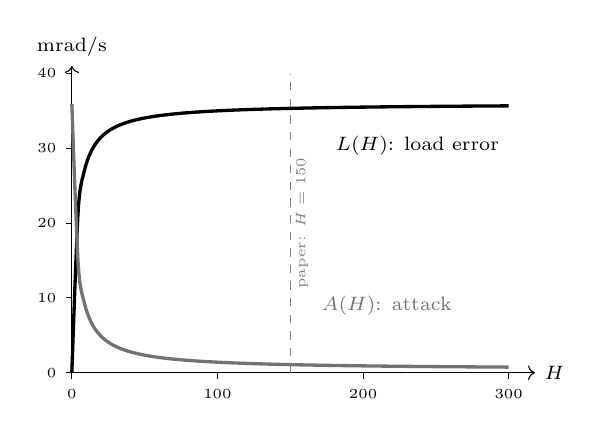
\begin{tikzpicture}[x=0.0185cm,y=0.095cm]
\draw[->] (0,0)--(318,0) node[right]{\scriptsize $H$};
\draw[->] (0,0)--(0,41) node[above]{\scriptsize mrad/s};
\foreach \h in {0,100,200,300}{\draw (\h,0)--(\h,-0.9) node[below]{\tiny \h};}
\foreach \v in {0,10,20,30,40}{\draw (0,\v)--(-4,\v) node[left]{\tiny \v};}
\draw[very thick,black,domain=0:300,samples=70,smooth] plot (\x,{36.02*\x/(\x+2.882)});
\draw[very thick,black!55,domain=0:300,samples=70,smooth] plot (\x,{0.4143*(\x+250)/(\x+2.882)});
\draw[dashed,gray] (150,0)--(150,40);
\node[font=\tiny,gray,rotate=90] at (158,20) {paper: $H=150$};
\node[font=\scriptsize,black,anchor=north east] at (300,33) {$L(H)$: load error};
\node[font=\scriptsize,black!55,anchor=west] at (165,9) {$A(H)$: attack};
\end{tikzpicture}
\end{center}
{\scriptsize Analytic curves, constant bias attack. Compare with Octave Fig.~4 (next slide).}
\end{columns}
\end{frame}

% =========================================================================
\begin{frame}[t]{[mine] Fig.~4: numerical $H$-sweep from the Octave script}
\begin{columns}[T]
\column{0.62\textwidth}
\figorbox{Fig4_Tradeoff_Curve.png}{1.0}
\column{0.36\textwidth}
\footnotesize
\begin{itemize}
\item Sweep of $H\in[10,300]$: load-step error (blue) rises and saturates near $3.5\times10^{-2}$; sinusoidal-attack peak (red) falls.
\item Numerical values (sin.\ attack, node 1): $H{=}10$: $1.2\times10^{-2}$; $50$: $3.2\times10^{-3}$; $150$: $1.5\times10^{-3}$; $300$: $1.0\times10^{-3}$\,rad/s.
\item $H=150$ sits on the \emph{flat} part: the load error is already saturated, while the attack peak is still falling slowly.
\end{itemize}
\begin{alertblock}{Do not claim}\scriptsize
A ``scissors crossing at the paper's $H=150$''. The crossing is at small $H$ (single digits).
\end{alertblock}
\end{columns}
\end{frame}

% =========================================================================
%  PART V
% =========================================================================
\begin{frame}[t]{Strengths}
\footnotesize
\begin{columns}[T]
\column{0.5\textwidth}
\begin{block}{Conceptual}
\begin{itemize}
\item \textbf{Detection-free resilience.} Bounded attacks are tolerated by structure (a leaky state), not by recognising them.
\item \textbf{Resilience as a number.} $\bar\delta$ from a small optimisation problem, in the same units as the attack, tied to a grid-code limit $\bar y$.
\item \textbf{Clean proof skeleton.} $\dot V=-\omega^TD\omega-\xi^T\bbH\xi$ (the skew coupling cancels) $+$ $\Lone$ gains $+$ small gain.
\end{itemize}
\end{block}
\column{0.48\textwidth}
\begin{block}{Practical}
\begin{itemize}
\item Retrofit of integral control; distributed implementation if $\bbK$ is a Laplacian and $\bbH$ diagonal.
\item Evidence beyond ideal simulation: parameter perturbation, replay, mixed SG/GFL grid, PHIL hardware tests.
\item My reduced-order check agrees with the mechanism: a leak bounds the effect of a bias on $\xi$ by orders of magnitude (about $40$--$70\times$ in the constant-bias $\delta_\xi$ rows).
\end{itemize}
\end{block}
\end{columns}
\end{frame}

% =========================================================================
\begin{frame}[t]{Limitations and critique}
\footnotesize
\begin{columns}[T]
\column{0.5\textwidth}
\textbf{1. Restoration is approximate by design.} $\omega_s=0$ is lost under any persistent mismatch (formula (c)). At the tested tuning the leak returns only $\approx1.9\%$ of the load error. The paper attributes the $<0.2\%$ offset to the VSG governor; the leak plausibly contributes too, but this cannot be separated at swing level.
\medskip

\textbf{2. Baselines vs.\ attack channel.} The paper does not say how the computational-attack analogue $\delta_\xi$ is applied to DAI/robust/primal-dual, so the comparison may not be like for like. In my reduced model, \emph{no} secondary loop beats the leaky one under bias attack ($4.1$ vs.\ $10.9\times10^{-4}$): the controller itself adds attack surface.
\medskip

\textbf{3. Scope of the attack model.} Additive, bounded, state-independent, on $u$ and $\xi$ only. Measurement/neighbour-exchange, DoS, replay, state-dependent (adaptive) attacks are excluded; Case 3 is simulation only.
\column{0.48\textwidth}
\textbf{4. Proof details.} $V$ is only semidefinite (angle shift invariance); Theorem 1 needs a continuation argument to justify $\gamma_\nu(\bar q)$; convexity of (23) is asserted via [41]; typos in (16)--(19).
\medskip

\textbf{5. Reproducibility.} $\Phi$, $\psi^*$, $\bar y$, and the actual $\bar\delta$ are not reported; no tuning guidance for $(\beta,\bbH)$ beyond ``large $\beta$ gives oscillation''.
\medskip

\textbf{6. Conservatism} (admitted): the $\Lone$ bound with elementwise worst-case combining is likely loose.
\medskip

\textbf{7. Equilibrium assumption.} $\xi^*=0$ presumes no net mismatch; load changes shift the leaky controller to $\xi^*\ne0,\ \omega^*\ne0$, outside the theory.
\end{columns}
\end{frame}

% =========================================================================
\begin{frame}[t]{Conclusion}
\footnotesize
\begin{columns}[T]
\column{0.55\textwidth}
\begin{block}{Take-aways}
\begin{enumerate}
\item The paper makes secondary frequency control \emph{tolerant} to bounded FDI by adding a leaky ancillary state, and certifies it with a Lur'e-form, $\Linf/\Lone$ small-gain analysis and a convex ``maximum attack'' program.
\item Mechanism, in one line: $u=-\beta^2K(sI+H)^{-1}K^T\omega$. The leak bounds the controller's response to injected bias; the price is exact restoration.
\item My reduced model confirms the mechanism and shows the cost: $\approx40$--$70\times$ less deviation than a pure integrator under constant bias, but only $\approx2\%$ restoration versus primary control at $H=150$.
\end{enumerate}
\end{block}
\column{0.43\textwidth}
\begin{alertblock}{Open questions}
\begin{itemize}
\item How should $(\beta,H)$ be chosen for a target mix of attack tolerance and restoration?
\item Can the leak be made adaptive, off when no attack is present?
\item Extension of the guarantee to measurement attacks, DoS, state-dependent attacks.
\item Less conservative certificates than $\Lone$ gains.
\end{itemize}
\end{alertblock}
\end{columns}
\vspace{0.2cm}
\centering\Large Thank you. Questions?
\end{frame}

% =========================================================================
%  APPENDIX
% =========================================================================
\appendix

\begin{frame}[t]{Appendix A: notation and symbol glossary}
\scriptsize
\begin{columns}[T]
\column{0.5\textwidth}
\begin{tabular}{@{}p{1.5cm}p{5.2cm}@{}}
\toprule
$\theta,\omega$ & angle, frequency deviation of IBRs\\
$M,D$ & inertia, damping (diagonal)\\
$P^{\rm net}$ & nominal power injection\\
$E$ & node--line incidence matrix ($n\times l$)\\
$\Phi$ & line weights $b_{ij}V_iV_j$ (diagonal)\\
$\psi^*$ & equilibrium angle differences $E^T\theta^*$\\
$q$ & $E^T(\theta-\theta^*)$, angle-difference error\\
$\nu(q)$ & nonlinear remainder of $\sin$\\
$\xi$ & ancillary controller state\\
$\beta,\bbK,\bbH$ & gain, interconnection matrix, leak\\
\bottomrule
\end{tabular}
\column{0.5\textwidth}
\begin{tabular}{@{}p{1.5cm}p{5.2cm}@{}}
\toprule
$\delta_u,\delta_\xi$ & actuation, computational FDI\\
$\bar\delta,\bar y,\bar q$ & bounds on attack, frequency, angle error\\
$\norm{\cdot}_{\Linf}$ & elementwise sup-norm (vector)\\
$\gamma_G$ & gain matrix, entries $\norm{G_{ij}}_{\Lone}$\\
$\gamma_\nu$ & diagonal gain of $\nu_i$\\
$E^T_{|\cdot|}$ & $E^T$ with absolute-value entries\\
$\lambda_{\max}$ & Perron--Frobenius eigenvalue\\
BIBO & bounded-input bounded-output\\
VSG, GFM, GFL & virtual synchronous gen., grid-forming, grid-following\\
DAI & distributed averaging integral control\\
PHIL & power hardware-in-the-loop\\
\bottomrule
\end{tabular}
\end{columns}
\end{frame}

% =========================================================================
\begin{frame}[t]{Appendix B: anticipated questions (1/3)}
\scriptsize
\textbf{Q1. Why simulate only the swing level, not LCL filters, inner loops and DC link like the paper?}\\
The paper's theory (Lur'e form, Lemmas 1--2, Theorem 1) is derived from (7) alone. Simulating (7) tests the control law and the theory without confounding inner-loop tuning. The price: I make no claim about full-order behaviour or about the baselines [14], [24], [47].
\medskip

\textbf{Q2. Does the pure integrator ``wind up to infinity''?}\\
Not in the frequency: with local integrators each $\omega_i$ is pinned near $\delta_{\xi,i}/(\beta K)$ (about $4.7\times10^{-2}$\,rad/s max). What grows is the \emph{angle drift}: the angle differences have no equilibrium and slip at a constant rate (see differential-mode slide). In the 7\,s window it is a frequency split; sustained, it would cost synchronism.
\medskip

\textbf{Q3. Why is the leak $\bbH\succ0$ needed in the proof?}\\
$\dot V=-\omega^TD\omega-\xi^T\bbH\xi$. With $\bbH=0$ the $\xi$ term disappears from $\dot V$: only $\omega$ is controlled, $\xi$ is free, and a bias on $\xi$ has no restoring force. With $\bbH\succ0$, $\xi$ is exponentially damped, which gives finite gains $\gamma$.
\medskip

\textbf{Q4. Why $\Linf$ and $\Lone$ rather than $\mathcal L_2$/$H_\infty$?}\\
Grid codes limit the \emph{peak} frequency. The $\Linf$-induced norm of an LTI system is the $\Lone$ norm of its impulse response (peak-to-peak gain), so the bound is both tight and computable elementwise.
\medskip

\textbf{Q5. The leaky controller never restores frequency to exactly 0; why call it secondary control?}\\
Correct, and my formula shows it: $\omega_s=[H(\bar\delta_u+\overline{\Delta P})+\beta K\bar\delta_\xi]/(HD+\beta^2K^2)$. It is a deliberate trade: exact integral action is exactly the component a bias attack exploits. At $H=150$ the restoration left is small ($\approx2\%$ of the load error).
\end{frame}

% =========================================================================
\begin{frame}[t]{Appendix B: anticipated questions (2/3)}
\scriptsize
\textbf{Q6. In your table, primary-only beats the proposed controller under attack. Doesn't that defeat the point?}\\
Yes in magnitude: a loop that does not exist cannot be attacked ($4.1\times10^{-4}$ vs.\ $10.9\times10^{-4}$ rad/s). But primary-only restores nothing (load error $3.60\times10^{-2}$). The paper's claim is relative to \emph{integral} secondary control, and my numbers support that ($\approx40$--$70\times$ better on $\delta_\xi$).
\medskip

\textbf{Q7. What if the attack exceeds the computed bound $\bar\delta$?}\\
The certificate is lost. Physically, the linear part stays BIBO stable but $|q|$ can exceed $\pi/2$ (Assumption 1), where the sine nonlinearity stops being a stabilising restoring force: synchronism can be lost. Unbounded attacks are excluded by Assumption 2.
\medskip

\textbf{Q8. What does $\beta$ do?}\\
From my formula the attack-induced deviation scales as $\sim\bar\delta_\xi/(\beta K)$ for large $\beta$, consistent with Fig.~3: larger $\beta$ tolerates larger attacks. The paper warns that too large a $\beta$ worsens oscillation (the common-mode poles move: $s^2+(D/M{+}H)s+(DH{+}\beta^2K^2)/M$).
\medskip

\textbf{Q9. Is (23) really convex?}\\
With $\gamma_\nu$ fixed it is linear in $(\bar\delta,\bar q)$. The dependence $\gamma_\nu(\bar q)$ is handled by citing [41] and the bound $|\psi_i^*|+\bar q_i\le\pi$; the paper does not prove it in situ.
\medskip

\textbf{Q10. How do you know your simulation is right?}\\
The leaky-controller constant-bias numbers agree with the closed-form steady-state formula to three digits, and with a separate Python implementation of the same ODE. The $H=0$ numbers cannot be checked in closed form (no synchronous steady state), only numerically.
\end{frame}

% =========================================================================
\begin{frame}[t]{Appendix B: anticipated questions (3/3)}
\scriptsize
\textbf{Q11. Why is the paper's Lyapunov function acceptable if it is not positive definite?}\\
$L_\psi$ has the kernel $\mathrm{span}(\ones)$. Define $V$ on $(q,\omega,\xi)$ or restrict to $\tilde\theta\perp\ones$; LaSalle then yields convergence to synchronisation. It is a presentational imprecision, not an error in substance.
\medskip

\textbf{Q12. Where does the paper's $0.2\%$ frequency offset come from?}\\
The paper: the VSG governor/power-sharing characteristic. My view: in the \emph{leaky} controller a persistent mismatch always leaves $\omega_s\ne0$ (formula (c)); the governor and leak effects cannot be separated without the full-order model.
\medskip

\textbf{Q13. Distributed implementation?}\\
Take $\bbK$ = Laplacian of the communication graph, $\bbH$ diagonal: each IBR needs only neighbour values. Note: with $\bbK$ \emph{diagonal} (as in the paper's test, $2I_4$) the controller is purely local.
\medskip

\textbf{Q14. Replay and DoS?}\\
Not covered by theory; Case 3 is a simulation of replayed signals (20-sample offset) with stable behaviour. The paper itself says no scheme resists all attacks (Remark 3).
\medskip

\textbf{Q15. Why does the baseline fail so dramatically in the paper but not in your model?}\\
I do not know; I did not reproduce the baselines. A plausible factor is the full-order dynamics and delays; another is the attack channel used for the baselines (see critique point 2). Say so rather than guess.
\end{frame}

% =========================================================================
\begin{frame}[t]{Appendix C: running the code (reference)}
\footnotesize
\begin{columns}[T]
\column{0.5\textwidth}
\textbf{Files in \texttt{\textasciitilde/projects/jamali-vsg/}}
\begin{itemize}
\item \texttt{jamali\_vsg\_demo.m}: main script: constant-bias table, load step, Figs.~1--4, saves PNGs.
\item \texttt{run\_sim.m}: segmented \texttt{ode45} integration with breakpoints $[0,2,5,12,T_{\rm end}]$ (events at load step and attack on/off).
\item \texttt{rhs\_func.m}: right-hand side of (7) plus attack and load-step logic.
\end{itemize}
\texttt{octave --no-gui jamali\_vsg\_demo.m}

Local functions at the end of a script file failed on this Octave version, hence the three files. \texttt{yyaxis} does not exist in Octave: Fig.~4 uses one axis.
\column{0.48\textwidth}
\textbf{Mapping code $\leftrightarrow$ paper}
\begin{center}
\begin{tabular}{@{}ll@{}}
\toprule
Code & Paper\\
\midrule
\texttt{M,D} & $M,D$ (Table I)\\
\texttt{E, Phi} & $E,\Phi$ (Phi assumed)\\
\texttt{beta, H} & $\beta,\bbH$ (6)\\
\texttt{K = 2*eye(4)} & $\bbK=2I_4$\\
\texttt{a(1:4), a(5:8)} & $\delta_u,\delta_\xi$ (7b,7c)\\
\texttt{dx(1:4)} & $\dot\omega$ in (7b)\\
\texttt{dxi} & $\dot\xi$ in (7c)\\
\bottomrule
\end{tabular}
\end{center}
\textbf{Compile this deck:} \texttt{pdflatex seminar.tex} (twice). Figures are read from the same folder.
\end{columns}
\end{frame}

% =========================================================================
\begin{frame}[t]{Appendix D: formula sheet}
\scriptsize
\begin{columns}[T]
\column{0.5\textwidth}
\textbf{Plant and controller}
\begin{align*}
\dot\theta&=\omega\\
M\dot\omega&=-D\omega+P^{\rm net}-E\Phi\sin(E^T\theta)+\beta\bbK\xi+\delta_u\\
\dot\xi&=-\bbH\xi-\beta\bbK^T\omega+\delta_\xi
\end{align*}
\textbf{Lur'e form:} $\dot x=Ax+B_\nu\nu(q)+B_\delta\delta,\ y=C_yx,\ q=C_qx$

\textbf{Lyapunov:} $V=\tfrac12\tilde\theta^TL_\psi\tilde\theta+\tfrac12\omega^TM\omega+\tfrac12\xi^T\xi$, $\dot V=-\omega^TD\omega-\xi^T\bbH\xi$

\textbf{Nonlinear gain:} $|\nu_i/q_i|\le|q_i|/2$
\column{0.5\textwidth}
\textbf{Small gain / bound}
\begin{align*}
\Gamma&=E^T_{|\cdot|}\gamma_{y,\nu}\gamma_\nu,\quad\lambda_{\max}(\Gamma)<1\\
\gamma&=\gamma_{y,\delta}+\gamma_{y,\nu}\gamma_\nu(I-\Gamma)^{-1}E^T_{|\cdot|}\gamma_{y,\delta}\\
\norm{y}_{\Linf}&\le\gamma\norm{\delta}_{\Linf}
\end{align*}
\textbf{Max attack:} $\max\bar\delta$ s.t. $E^T_{|\cdot|}(\gamma_{y,\delta}\bar\delta+\gamma_{y,\nu}\gamma_\nu\bar q)\le\bar q$,\ $\gamma_{y,\delta}\bar\delta+\gamma_{y,\nu}\gamma_\nu\bar q\le\bar y$

\textbf{[mine] Steady state (leaky, scalar gains):}
\[\omega_s=\frac{H(\bar\delta_u+\overline{\Delta P})+\beta K\bar\delta_\xi}{HD+\beta^2K^2}\]
Effective droop: $D_{\rm eff}=D+\beta^2K^2/H$. Common-mode poles: $Ms^2+(D{+}MH)s+DH+\beta^2K^2=0$.
\end{columns}
\end{frame}

\end{document}
